\ifdefined\isinprint
\documentclass[twoside,10pt]{book}
\usepackage[twoside,paperwidth=155.93mm,paperheight=233.89mm,hmargin={15mm,15mm},vmargin={20mm,20mm},bindingoffset=5mm]{geometry}
\usepackage[hyphens]{url} 
\usepackage[colorlinks=false,
            pdfborder={0 0 0}
	        pdftex,
            plainpages=false,
            pdfauthor={Lukas Ladenberger (Editor)},
            pdftitle={BMotion Studio User's Handbook},
            pdfsubject={BMotion Studio},
            pdfkeywords={ProB, Event-B},
            pdfproducer={http://www.stups.hhu.de/ProB/index.php5/BMotion_Studio},
            pdfcreator={plastex-based tool chain}]{hyperref}
\else
\documentclass[12pt]{book}
\usepackage[left=2.5cm,top=3cm,right=2.5cm,bottom=3cm]{geometry}
\usepackage[hyphens]{url} 
\usepackage[colorlinks=true,
	        pdftex,
            plainpages=false,
            pdfauthor={Lukas Ladenberger (Editor)},
            pdftitle={BMotion Studio User's Handbook},
            pdfsubject={BMotion Studio},
            pdfkeywords={ProB, Event-B},
            pdfproducer={http://www.stups.hhu.de/ProB/index.php5/BMotion_Studio},
            pdfcreator={plastex-based tool chain}]{hyperref}
\fi
\usepackage{graphicx}
\usepackage{bsymb}
\usepackage{b2latex}
\usepackage{fancyhdr,lastpage,color}
\usepackage{verbatim}
\usepackage{wrapfig}
\usepackage{makeidx}
\usepackage{fix-cm}
\usepackage[utf8]{inputenc}

\usepackage{listings}

\usepackage{longtable}

\lstdefinelanguage{Groovy}% 
{morekeywords={abstract,any,as,boolean,break,byte,case,catch,char,class, 
const,continue,def,default,do,double,else,extends,false,final,finally, 
float,for,goto,if,implements,import,instanceof,in,int,interface,label, 
long,native,new,null,package,private,protected,public,return,short, 
static,strictfp,super,switch,synchronized,this,throw,throws,transient, 
true,try,void,volatile,while,with},% 
sensitive=true,% 
morecomment=[l]//,% 
morecomment=[s]{/}{/},% 
morestring=[b]",% 
morestring=[b]',% 
}[keywords,comments,strings]
%
%\lstdefinelanguage{B}% 
%{morekeywords={MACHINE, REFINEMENT,OPERATIONS,INITIALISATION,END,BEGIN,PRE,IF,THEN,ELSE,VARIABLES,INVARIANT,SETS},% 
%sensitive=true,% 
%morecomment=[l]//,% 
%morecomment=[s]{/}{/},% 
%morestring=[b]",% 
%morestring=[b]',% 
%}[keywords,comments,strings]
%
%\lstset{
%  language={Java},basicstyle=\ttfamily\small,,columns=fullflexible
%}
%\lstset{
%  language={Groovy},basicstyle=\ttfamily\small,,columns=fullflexible
%}
%\lstset{
% numberbychapter=false
%}

\lstdefinelanguage{JavaScript}{
  keywords={typeof, new, true, false, catch, function, return, null, catch, switch, var, if, in, while, do, else, case, break},
  keywordstyle=\color{magenta}\bfseries,
  ndkeywords={class, export, boolean, throw, implements, import, this},
  ndkeywordstyle=\color{magenta}\bfseries,
  identifierstyle=\color{black},
  sensitive=false,
  comment=[l]{//},
  morecomment=[s]{/*}{*/},
  commentstyle=\color{purple}\ttfamily,
  stringstyle=\color{blue}\ttfamily,
  morestring=[b]',
  morestring=[b]"
}


\lstset{
  frame=top,frame=bottom,
  %basicstyle=\small\normalfont\sffamily,    % the size of the fonts that are used for the code
  stepnumber=1,                           % the step between two line-numbers. If it is 1 each line will be numbered
  numbersep=10pt,                         % how far the line-numbers are from the code
  tabsize=2,                              % tab size in blank spaces
  extendedchars=true,                     %
  breaklines=true,                        % sets automatic line breaking
  captionpos=t,                           % sets the caption-position to top
  mathescape=false,
  stringstyle=\color{blue}\ttfamily, % Farbe der String
  keywordstyle=\color{magenta}\ttfamily, % Farbe der String
  showspaces=false,           % Leerzeichen anzeigen ?
  showtabs=false,             % Tabs anzeigen ?
  xleftmargin=17pt,
  framexleftmargin=17pt,
  framexrightmargin=17pt,
  framexbottommargin=5pt,
  framextopmargin=5pt,
  showstringspaces=false,      % Leerzeichen in Strings anzeigen ?
  escapechar=\%,
  numbers=left,                    % where to put the line-numbers; possible values are (none, left, right)
  numbersep=5pt
 }

% Rodin Handbook Version Path. "current" is the newest version of the handbook. This should be changed if we want to build a handbook for another (i.e. older version)
\newcommand{\versionpath}{nightly}

% Absolute path to handbook
\newcommand{\handbookpath}{http://nightly.cobra.cs.uni-duesseldorf.de/bmotion/bmotion-prob-handbook}

\newcommand{\bms}{BMotion Studio}

% We generate an index
\makeindex


% defining a if(plastex) environment
\newif\ifplastex
\plastexfalse

% defining a if(isinprint) environment
\newif\ifinprint
\ifdefined\isinprint
\inprinttrue
\else
\inprintfalse
\fi

% for the print, we use an extra b&w directory
\ifinprint
\newcommand{\rodinimgdir}{img-print}
\else
\newcommand{\rodinimgdir}{img}
\fi

\ifinprint
\def\doculist#1#2{
\begin{quote}
\hspace{-10mm}
\includegraphics[height=4ex]{#2}
\vspace{-8mm}

#1
\end{quote}
}
\else
\def\doculist#1#2{
\begin{quote}
\hspace{-10mm}
\textrm{\includegraphics[width=7mm]{#2}} % Hack!  We "mark" the image with textrm so that we can use a different CSS-Style in plastex.
\vspace{-8mm}

#1
\end{quote}
}
\fi

% dimensions on the title page
\newlength{\titletop}
\newlength{\titlesubtitledistance}
\newlength{\titlebottom}
\newlength{\titlesecdistance}
\ifinprint
\def\titledimrodin{\fontsize{30}{50}}
\def\titledimhandbook{\fontsize{20.5}{25}}
\def\titledimsubtext{\fontsize{13}{16}}
\def\titledimsponsor{\fontsize{11}{15}}
\setlength{\titletop}{120mm}
\setlength{\titlesubtitledistance}{2mm}
\setlength{\titlebottom}{-30mm}
\setlength{\titlesecdistance}{8mm}
\else
\def\titledimrodin{\fontsize{40}{50}}
\def\titledimhandbook{\fontsize{24.5}{30}}
\def\titledimsubtext{\fontsize{16}{19}}
\def\titledimsponsor{\fontsize{11}{15}}
\setlength{\titletop}{145mm}
\setlength{\titlesubtitledistance}{2mm}
\setlength{\titlebottom}{-22mm}
\setlength{\titlesecdistance}{10mm}
\fi

\def\tick#1{\doculist{#1}{img/tick_64.png}}
\def\info#1{\doculist{#1}{img/info_64.png}}
\def\warning#1{\doculist{#1}{\rodinimgdir/warning_64.png}}
\def\pencil#1{\doculist{#1}{\rodinimgdir/pencil_64.png}}

% macro for icons
\def\icon#1{
\includegraphics[height=2ex]{\rodinimgdir/icons/#1}
}

% macro for image versions (pdf version + html version)
% #1 Path to image for pdf version
% #2 Path to image for html version
% #3 Caption
% #4 Label
\def\imagedpi#1#2#3#4#5{
	\ifplastex
		\begin{figure}[!ht]
		\begin{center}
			\includegraphics{#3}
			\caption{#4}
			\label{#5}
		\end{center}
		\end{figure}
	\else
		\begin{figure}[!ht]
		\begin{center}
			\includegraphics[width=#2]{\rodinimgdir/#1}
			\caption{#4}
			\label{#5}
		\end{center}
		\end{figure}
	\fi
}

\newcommand{\includerodinimg}[1]{\includegraphics{\rodinimgdir/#1}}
\newcommand{\includerodintwimg}[2]{\includegraphics[width=#1\textwidth]{\rodinimgdir/#2}}

% different method to write an ASCII backslash for plastex and normal pdflatex
\ifplastex
  \newcommand{\mybackslash}{\textbackslash}
\else
  % we do not use textbackslash for latex, because it does not use the current font setting
  \newcommand{\mybackslash}{\symbol{`\\}}
\fi

% Path to resources like zip's with machines
% We use a relative path in the html + eclipe version (in order to work offline)
% and an absolute path in the pdf version
\ifplastex
	\newcommand{\filepath}{files/}
    \newcommand{\file}[2]{\href{\filepath#1}{#2}}
\else
	\newcommand{\filepath}{\handbookpath/\versionpath/files/}
%    \newcommand{\file}[2]{\href{\filepath#1}{#2}\footnote{The URL of the resource is: \url{\filepath#1}}}
    \newcommand{\file}[2]{\href{\filepath#1}{#2}}
\fi

% Use this definition to create a link to the file. The definition takes to arguments. 
% The first argument (1) defines the file name i.e. Celebrity.zip or in case if you saved 
% the file in a subdirectory subdirecotry/Celebrity.zip. The second argument (2) defines 
% the name which should be displayed in the document, i.e. Celebrity Problem Example Download
%\def\file#1#2{
%\href{\filepath#1}{#2}
%}

% We want to mark contributions from other plugins in a special way, by including the plugin's
% icon and by putting the content in a gray box.  We have to approach this differently for
% Latex and for Plastex:
% Latex: We use "shaded" from package "framed"
% Platexte: We use "verse" as the marker and create the shading with the style sheet.
\newcommand{\tmpName}{Dummy}
\ifplastex
\newenvironment{rodin-plugin}[2]
{
\renewcommand{\tmpName}{#2}
  \begin{verse}
\begin{wrapfigure}{l}{}
    \includegraphics{\rodinimgdir/#1}
\end{wrapfigure}
}
{
\newline
\textit{This contribution requires the \textbf{\tmpName} plugin.  The content is maintained by the plugin contributors and may be out of date.}
\end{verse}
}
\else
\usepackage{framed}
\definecolor{shadecolor}{rgb}{0.93,0.93,0.93}
\newenvironment{rodin-plugin}[2]
{
\renewcommand{\tmpName}{#2} % Otherwise we cannot use #2 in the end block - stupid!
\begin{shaded}
\begin{wrapfigure}{l}{10mm}
\vspace{-5mm}
\includegraphics[width=10mm]{\rodinimgdir/#1}
\vspace{-5mm}
\end{wrapfigure}
\noindent
}
{
\vspace{1mm}
\noindent\rule{\textwidth}{.1pt}
\vspace{1mm}
\noindent
{\scriptsize This contribution requires the \textbf{\tmpName} plugin.  The content is maintained by the plugin contributors and may be out of date.}

\end{shaded}
}
\fi

\newenvironment{plugin-pror}{\begin{rodin-plugin}{pror.png}{ProR Requirements}}{\end{rodin-plugin}}

% Marginpars are  cropped - this formats them nicely.
\let\oldmarginpar\marginpar
\renewcommand\marginpar[1]{\-\oldmarginpar[\raggedleft\scriptsize{#1}]
{\raggedright\small{#1}}}
\marginparwidth=2cm

% A command to typeset names of an Event-B section (like variables, invariant, etc)
% consistently.
\newcommand{\eventbsection}[1]{\textsl{#1}}

% A command to typeset consistently the names of proof obligations
\newcommand{\eventbpo}[1]{\textsf{#1}}

% Event-B's finite operator
\newcommand{\bfinite}{\mathrm{finite}}
\newcommand{\bpartition}{\mathrm{partition}}
\newcommand{\bunaryunion}{\mathrm{union}}
\newcommand{\bunaryinter}{\mathrm{inter}}
% TODO: refactor the following command if needed
\newcommand{\boftype}{\mathbin{\raisebox{0.6ex}{\ensuremath{\circ}}\mkern-9mu\raisebox{-0.6ex}{\ensuremath{\circ}}}}

% Commands for the structure of the reference section

% rrnames is used for the array of operator symbols and description
% at the beginning of a reference section.
% The environment defines an array with three columns:
% 1) The mathematical symbol
% 2) The ASCII representation
% 3) A description of the operator
\newenvironment{rrnames}%
  {\begin{center}\begin{tabular}{l@{\quad---\quad}l@{\quad---\quad}l}}%
    {\end{tabular}\end{center}}

% The environment rodinrefentry is used for a reference section with several
% entries: Description, Definition, Types, Well-Definedness
% \rrindent is the indention in such an environment
\newlength{\rrindent}
\setlength{\rrindent}{8em}
\newenvironment{rodinrefentry}{%
   \renewcommand\descriptionlabel[1]{\makebox[\rrindent][r]{\textbf{##1}}}
   \setlength{\leftmargini}{\rrindent}
   \begin{description}%
}{%
   \end{description}%
   \pagebreak[3]%
}
\newcommand{\rrdesc}{\item[Description]}
\newcommand{\rrdef}{\item[Definition]}
\newcommand{\rrtypes}{\item[Types]}
%\newcommand{\rrwd}{\item[Well-Definedness]}
\newcommand{\rrwd}{\item[WD]}
\newcommand{\rrfis}{\item[Feasibility]}
\newcommand{\rrex}{\item[Example]}

% feasibility of actions as operator
\newcommand{\actfis}{\mathcal{F}}

% free identifiers in an expression
\newcommand{\freeids}[1]{\textsl{Free}(#1)}

% placeholder for arbitrary expressions
\newcommand{\vexpr}[1]{\textsf{#1}}
\newcommand{\predp}{\vexpr{P}}
\newcommand{\predq}{\vexpr{Q}}
\newcommand{\expra}{\vexpr{A}}
\newcommand{\exprb}{\vexpr{B}}
\newcommand{\expre}{\vexpr{E}}
\newcommand{\exprf}{\vexpr{F}}
\newcommand{\exprr}{\vexpr{R}}
\newcommand{\exprs}{\vexpr{S}}
\newcommand{\exprt}{\vexpr{T}}
\newcommand{\exprla}{\vexpr{a}}
\newcommand{\exprlb}{\vexpr{b}}
\newcommand{\exprle}{\vexpr{e}}
\newcommand{\exprlf}{\vexpr{f}}
\newcommand{\exprlp}{\vexpr{p}}
\newcommand{\exprlr}{\vexpr{r}}
\newcommand{\exprls}{\vexpr{s}}

% operators (L and D) for well-definendness
\newcommand{\wdl}{\mathcal{L}}
\newcommand{\wdd}{\mathcal{D}}

% a placeholder symbol for operators
\newcommand{\opelipse}{\mathbin{\Box}}

% a second approach to proof obligations
\newcommand{\pode}[3]{%
  \begin{center}
    \setlength{\parindent}{2em}\vspace{0.2em}
    \begin{tabular}{rp{0.6\textwidth}}
      \hline
      & \textbf{#1} \\
      Name       & #2 \\
      Goal       & #3 \\
      \hline
    \end{tabular}
  \end{center}
}


% Titlepage stuff
\ifplastex
\else

\usepackage{eso-pic}
\newcommand\BackgroundPic{
\put(0,0){
\parbox[b][\paperheight]{\paperwidth}{%
\vfill
\centering
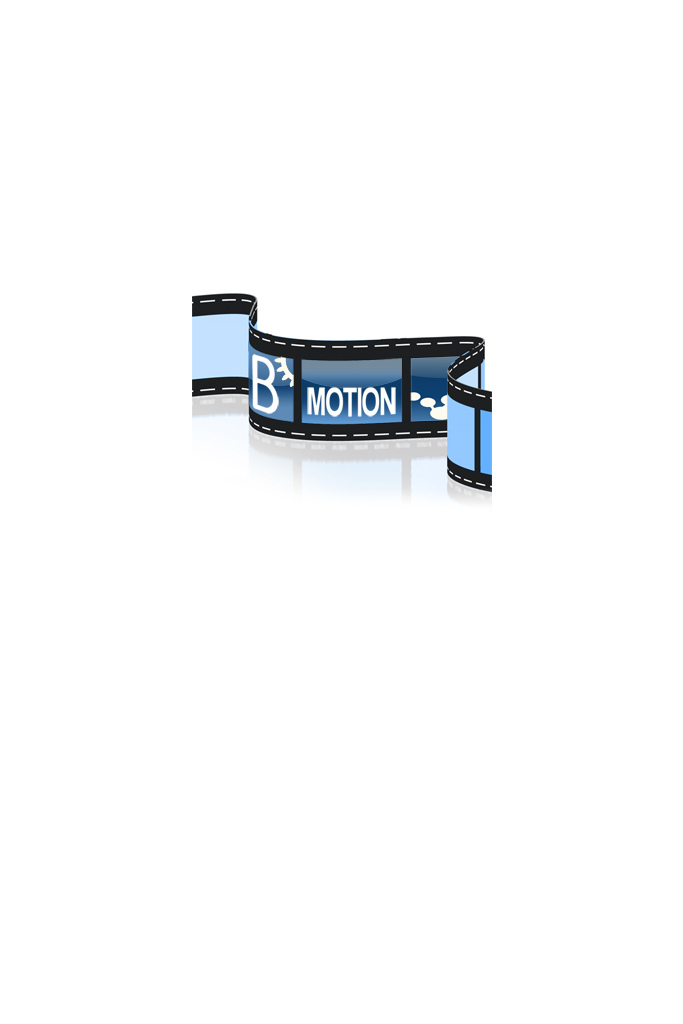
\includegraphics[width=\paperwidth,
keepaspectratio]{img/bms-handbook-bg.jpg}%
\vfill
}}}

\fi

%%% Local Variables: 
%%% mode: latex
%%% TeX-master: "rodin-doc"
%%% End: 


\title{BMotion Studio User's Handbook}
\author{
Work in Progress\\
Handbook $ $Rev: 16185 $ $ \\
\\
\href{mailto:ladenberger@cs.uni-duesseldorf.de}{ladenberger@cs.uni-duesseldorf.de}\\
\href{http://www.stups.hhu.de/ProB/index.php5/BMotion_Studio}{http://www.stups.hhu.de/ProB/index.php5/BMotion_Studio}
}

\begin{document}        
\pagestyle{empty}
\ifplastex
\maketitle
\else
\pagenumbering{roman}
\begin{titlepage}
\AddToShipoutPicture*{\BackgroundPic}
\vspace*{\titletop}
{\titledimrodin\selectfont \bfseries BMotion Studio}

\vspace*{\titlesubtitledistance}
{\titledimhandbook\selectfont \bfseries User's Handbook}

\vspace*{\titlesecdistance}
{\titledimsubtext\selectfont \textbf{\textsf{ProB Edition}}}

\vspace*{\titlesecdistance}
{\titledimsubtext\selectfont \textsf{Lukas Ladenberger (Editor)}}

\vspace*{\titlesecdistance}
{\titledimsponsor\selectfont %
  $\hbox{
\includegraphics[height=4ex]{img/advance-logo.png}}$
  \textsf{This work is sponsored by the ADVANCE Project}}

\vspace*{\titlebottom}

\end{titlepage}
\ifdefined\isinprint
\cleardoublepage
% Title page
\vspace*{10em}
\begin{center}
  {\huge \textbf{BMotion Studio User's Handbook}}\\
  \vspace{2em}
  {\large ProB Edition}
\end{center}
\clearpage
% Copyright page
\vspace*{\fill}
\noindent\textbf{BMotion Studio User's Handbook}\\
~\\
This work, except the cover image, is licensed under the Creative Commons Attribution-ShareAlike 3.0 Unported License. To view a copy of this license, visit \href{http://creativecommons.org/licenses/by-sa/3.0/}{creative\-com\-mons.org/\-licenses/\-by-sa/3.0/} or send a letter to Creative Commons, 444 Castro Street, Suite 900, Mountain View, California, 94041, USA.\\
The cover image of a Rodin statue was created by Miikka Skaffari.
It is licensed under a Creative Commons Attribution-NonCommercial 3.0 Unported License.  To view a copy of this license, visit \href{http://creativecommons.org/licenses/by-sa/3.0/}{creative\-com\-mons.org/\-licenses/\-by-sa/3.0/} or send a letter to Creative Commons, 444 Castro Street, Suite 900, Mountain View, California, 94041, USA.
\vspace{10em}
\else\fi
\cleardoublepage
\pagenumbering{arabic}
\phantomsection
\addcontentsline{toc}{chapter}{Contents}
\tableofcontents
\fi

\chapter{Introduction}
\label{introduction}

\section{Overview}

This handbook consists of five parts:

\begin{description}
	\item[Introduction (Chapter~\ref{introduction})] You are reading the introduction right now.  Its purpose is to help you orient yourself and to find information quickly.
	\item[Tutorial (Chapter~\ref{tutorial})] If you are completely new to BMotion Studio, the tutorial is a good way to get up to speed quickly.  It guides you through the installation and usage of the tool.
	\item[Reference (Chapter~\ref{reference})] The reference section provides comprehensive documentation of BMotion Studio and its components.
	\item[Frequently Asked Questions  (Chapter~\ref{faq})] Common issues are listed by category in the FAQ.
	\item[Index] We included an index particularly for the print version of the handbook, but it may be useful in the electronic versions as well.  
\end{description}

\subsection{Formats of this Handbook}
\label{handbook_formats}

The handbook comes in various formats:

\begin{description}
	\item[Online Help] You can access the handbook online at \url{http://www.stups.hhu.de/ProB/index.php5/BMotion_Studio}.
	\item[PDF Help] Both online versions also include a link to the PDF version of the handbook.
\end{description}

\section{Conventions}
\label{conventions}

We use the following conventions in this manual:

\tick{Checklists and milestones are designated with a tick. Here we summarize what we want to learn or should have learned so far.}
\info{Useful information and tricks are designated by the information sign.}
\warning{Potential problems and warnings are designated by a warning sign.}
\pencil{Examples and Code are designated by a pencil.}

We use \texttt{typewriter} font for file names and directories.

We use \textsf{sans serif font} for GUI elements like menus and buttons.  Menu actions are depicted by a chain of elements, separated by ``$\rangle$'', e.g. \textsf{File $\rangle$ New $\rangle$ Visualisation}.

\section{ADVANCE}
\label{advance}

This work has been sponsored by the Advance project\footnote{\url{http://www.advance-ict.eu/}}.  ADVANCE is an FP7 Information and Communication Technologies Project funded by the European Commission. The overall objective of ADVANCE is the development of a unified tool-based framework for automated formal verification and simulation-based validation of cyber-physical systems.

The ADVANCE project is unique in addressing both simulation and formal verification within a single design framework.

Unification is being achieved through the use of a common formal modelling language supported by methods and tools for simulation and formal verification. An integrated tool environment is providing support for construction, verification and simulation of models.

ADVANCE is building on an existing formal modelling language - Event-B - and its associated tools environment - Rodin - with strong support for formal verification. In ADVANCE, Rodin is being further strengthened and augmented with novel approaches to multi-simulation and testing.

\section{Creative Commons Legal Code}
\label{sec:cc}        

The work presented here is the result of an collaborative effort
that took many years.  To ensure that access to this work stays free
and to avoid any legal ambiguities, we decided to formally lincense
it under the Creative Commons Share-Alike License.

This work is licensed under the Creative Commons Attribution-ShareAlike 3.0 Unported License. To view a copy of this license, visit \url{http://creativecommons.org/licenses/by-sa/3.0/} or send a letter to Creative Commons, 444 Castro Street, Suite 900, Mountain View, California, 94041, USA.



% \section{Style Guide}
\label{style-guide}

\info{For now, we will manage the style guide as a \LaTeX~document together with the rest of the documentation.  We may take it out upon publication.}

\subsubsection{General Stylistic Guidelines}

\begin{itemize}
	\item The conventions (\ref{conventions}) are part of the style guide.

	\item Use the ``we'' form.

	\item We use British English.

	\item When referring to the different views in Rodin, the word ``view'' should be written in lowercase, e.g., the Rodin Problems view.
\end{itemize}

\subsubsection{Files}

Files should be saved in the \texttt{files} subdirectory. You can also create a subdirectory. Then, use the definition 

\begin{verbatim} \file{1}{2} 
\end{verbatim} 

to create a link to the file. The definition extends to arguments. The first argument (1) defines the file name i.e. \texttt{Celebrity.zip} or if you saved the file in a subdirectory \texttt{subdirectory/Celebrity.zip}. The second argument (2) defines the name which should be displayed in the document, i.e. ``Celebrity Problem Example Download''.

\warning{Please note, that you only enter the file name without a path before (expected subdirectories). The build script assigns the correct path to the file on the server automatically .}

Here is an example using the definition: \file{Celebrity.zip}{Celebrity Problem Example Download}.

\subsubsection{Avoiding Redundancy}

We will reduce (or avoid) redundancy through heavy linking, following these guidelines:

\begin{itemize}
	\item If in doubt, provide the bulk of the information in the Reference section.  For instance, the FAQ entry ``What is Event-B?''  Should simply refer to the Event-B entry in the Reference section.
	\item Web Links should not appear multiple times
	\item List web links as footnotes in the Tutorial and FAQ.
	\item List web links in a ``See also'' Section in the Reference.
\end{itemize}

\subsubsection{Sections}

\begin{itemize}
	\item If referring to a specific chapter or section, use uppercase to denote it, e.g. ``in Chapter~3''.
	\item We also refer to subsections as Section, e.g. ``see Section~2.5''
	\item We have a small number of well-defined chapters which are the top level structuring element.
	\item Sections and subsections are numbered.  In the HTML-Versions, they are broken into subpages.
    \item Subsubsections do not receive numbers and are not broken into subpages in the HTML.  Keep this in mind regarding both the reading flow and page sizes.
	\item Avoid linking (ref) to subsubsections, as they don't have a number.  Latex will instead provide a link to the next higher element.  This works, but it could create confusion.
	\item Generally, we should avoid gaps in the hierarchy (i.e. having a subsubsection in a section without a subsection in between).\footnote{Coincidentally, this style guide violates this rule. Reason: We want the style guide to remain whole and not be broken into subsections, but the proper hierarchy is a section.}
	\item Section labels should be all in lower case. Use ``\_'' for blanks.
	\item We use the prefix ``\texttt{int\_}'' for introduction section labels, ``\texttt{tut\_}'' for tutorial section labels following a meaningful description of the section (i.e. \texttt{tut\_rodin\_installation}) and ``\texttt{faq\_}'' for faq section labels following a short version of the title (i.e. \texttt{faq\_diff\_eventb\_b}). Reference section labels have no prefix.
\end{itemize}

\subsubsection{Images}
\begin{itemize}
	\item Images must be no more than 700 pixels in width (for HTML version) and no more than 160 mm (for PDF version). This is fairly easy for bitmaps (screenshot), pay attention to this regarding how plasTeX converts vector images. (see Latex section below on how to include images)

	\item Screenshots should look neat and consistent.  Horizontal real estate will always be an issue, so please resize the windows before taking the screenshot to keep things readable at 700 pixel width.  (see Latex section below on how to include images)

	\item Images should always have a caption and a label. Please use the same conventions for the figure labels that are used for the the section labels, but use the prefix ``\texttt{fig\_}''. \\Example: ``\texttt{fig\_tut\_03\_traffic\_light}''. For referencing do not use references like "As shown bellow" or "Like in the following image:". Use always a format like:

\begin{verbatim}"... as shown in figure \ref{fig_tut_03_traffic_light}."\end{verbatim}

	\item We use icons from Pixel-Mixer, which are free as long as credit is given: \url{http://www.softicons.com/free-icons/toolbar-icons/basic-icons-by-pixelmixer}

  \item We include Window decoration only when it is really necessary.  If we discuss only some views, we crop the rest away.  Please crop neatly, following edges. Even if you need a screenshot with window decoration, you should always use the same Window decoration (i.e. linux ubuntu default decoration style). If you need such a screenshot, please contact Lukas.

  \item Image file names should be all in lower case and not include umlaute or special characters. Use ``\_'' for blanks.

  \item Image files should keep the following rules:
	
\begin{itemize}
		\item Tutorial images should be saved in the sub folder \texttt{img/tutorial} with the prefix ``\texttt{tut\_}'' following the section number. For instance, \texttt{tut\_01\_image1.png}.

		\item FAQ images should be saved in the sub folder \texttt{img/faq} with the prefix ``\texttt{faq\_}''. For instance, \texttt{faq\_image1.png}.

	\end{itemize} 
	\end{itemize}

\subsubsection{Icons}

For icons (i.e. RODIN platform icons) in continuous text use the command: 

\begin{verbatim} \icon{1} \end{verbatim} 

The first (1) argument takes the path to the icon (i.e. \texttt{rodin/auto\_prover.png}). You can find all icons in the folder \texttt{latex/img/icons/}

Here is an example using icons in continuous text:

\textit{Lorem ipsum dolor sit amet, consetetur \icon{rodin/auto_prover.png} sadipscing elitr, sed diam nonumy eirmod tempor invidunt ut labore et dolore magna aliquyam erat, sed diam voluptua. At vero eos et accusam et justo duo dolores et ea rebum. Stet clita kasd gubergren, no sea takimata sanctus est Lorem ipsum dolor sit amet. Lorem ipsum dolor sit amet, consetetur sadipscing elitr, sed diam nonumy eirmod tempor invidunt ut labore et dolore \icon{rodin/lasoo_prover.png} magna aliquyam erat, sed diam voluptua. At vero eos et accusam et justo duo dolores et ea rebum. Stet clita kasd gubergren, no sea takimata sanctus est Lorem ipsum dolor sit amet.}

\subsubsection{Index}
Please add meaningful entries to the index. This helps users to look up information more efficiently.
The \LaTeX-command to do this is \verb#\index{#\textit{word}\verb#}#.
\begin{itemize}
\item The most important thing to think about when considering the index is the user perspective: 
  What is the word that a user will look up to try and find this topic?
\item An index entry should be a noun, singular and written in lowercase (uppercase if it's a name).
\item If the word appears in are several locations in the documentation (e.g. in the tutorial and the
  reference section), try to highlight the most commonly used location with \verb#\index{word|textbf}#.
  This is usually an entry in the reference section.
\item Adjectives should be used with care. 
  Please use them only if omitting the adjective changes the meaning of the entry drastically or
  if the adjective is necessary to distinguish the entry from other entries with the same noun but
  other location.
\item If you use an adjective, consider using the noun as a key for sorting: \verb#\index{cloud,grey@grey cloud}#
  instead of \verb#\index{grey cloud}#
\item If you have multiple entries for the same word, consider using sub-entries (\verb#\index{cloud!grey}#)
  if different things are meant. Another example is \verb#\index{true!as predicate}# and \\ \verb#\index{true!as expression}#
\item Multiple index entries for the same text block are alright.
\item If you use the index command, please have a look at the result.
\end{itemize}

\subsubsection{\LaTeX{} Styling}

\begin{itemize}
	\item Try to avoid fancy \LaTeX formatting, as PlasTeX (used for generating HTML) is temperamental.  Macros are especially problematic, and sometimes the result is just ugly.
	\item We have the option to use different files to generate the PDF and HTML, but we would generally prefer not to do this.  Look at \texttt{bsymb.sty} and \texttt{plastex-bsymb.sty} as an example. \textbf{NOTE:} We don't do this any more for any style files.
	\item Every section should have a label, reflecting the section name, all lowercase, spaces replaced with underscores (\_).
	\item Don't create subdirectories in the \texttt{latex} folder, as the scripts cannot always deal with them.
	\item Put images in the \texttt{img} folder.  Feel free to create additional directory structures underneath.
	\item Files other than images (e.g. Event-B projects) --- we have macros to link them absolute in the PDF, and to link them relative in HTML and Eclipse Help.
	\item Use linked sections numbers (generated with \texttt{\\ref{}} instead of hyperlinks for cross-references. This is necessary for the print documentation to be useful.
	\item When including images in Latex, do not provide a width!  Instead, try to embed the print size in the image itself.  For instance, PNGs allow you to set the print size (in mm).  This way we can be sure that the images are rendered as HTML without distortion.
\end{itemize}

\subsubsection{Contributions from Plugin Developers}
\label{sec:plugin_contributions}

\begin{rodin-plugin}{prob.png}{ProB}
We want to encourage Plugin developers to contribute to the Handbook, but we have to make it clear that we cannot maintain that documentation.  Therefore, it has to be clearly marked.  We use a custom environment for that purpose that
(1) provides the Plugin's icon, (2) adds a disclaimer to the end of the custom documentation and (3) puts the content into a gray box (like this one).

There are some limitations to the environment that we use.  Specifically, headlines and images should be kept outside the gray box.

\end{rodin-plugin}

%%% Local Variables: 
%%% mode: latex
%%% TeX-master: "rodin-doc"
%%% End: 


\chapter{Tutorial}
\label{tutorial}


The objective of this chapter is to get you to a stage where you can use BMotion Studio to visualize formal models.  
We expect you to have a basic understanding of logic and an idea why doing formal modelling is a good idea.  
You should be able to work through the tutorial with no or little outside help.

This tutorial covers installation and configuration of BMotion Studio; it brings you through step by step through building visualizations for formal models and it provides the essential theory and provides pointers to more information.

We attempt to alternate between theory and practical application thereby keeping you motivated.  
We encourage you not to download solutions to the examples but instead to actively build them up yourself as the tutorial progresses.

If something is unclear, remember to check the Reference (\ref{reference}) for more information.

\section{Outline}

\begin{description}
	\item[Background before getting started (\ref{tutorial_01})] We give a brief description of what BMotion Studio is and what it is being used for and what kind of background knowledge we expect.
	\item[Installation and first steps (\ref{tutorial_02})] We guide you through downloading, installing and starting BMotion Studio. 
	\item[We create our first visualisation (\ref{tutorial_03})] We are going to create our first visualization for a simple lift Event-B model. 
	
\end{description}


\section{Before Getting Started}
\label{tutorial_01}

What is BMotion Studio?

(tbd)

Before we get started with the actual tutorial, we are going to go over the required background to make sure that you have a rudimentary understanding of the necessary concepts.

\tick{\textbf{You can skip this section, if...}
\begin{itemize}
	\item ... you know what formal modelling is
	\item ... you know what predicate logic is
	\item ... you know what ProB refer to
\end{itemize}
}

\subsection{Formal Modelling}

We are concerned with \textit{formalizing specifications}.  This allows us a more rigorous analysis (thereby improving the quality) and allows the reuse of the specification to develop an implementation.  This comes at the cost of higher up-front investments.

This differs from the traditional development process. In a formal development, we transfer some effort from the test phase (where the implementation is verified) to the specification phase (where the specification in relation to the requirements is verified).

\subsection{Predicate Logic}
\label{predicate_logic}
\index{predicate logic}

Predicate logic is a mathematical logic containing variables that can be quantified.

Event-B supports first-order logic which is, technically speaking, just one type of predicate logic.  

\subsection{Event-B}
\label{eventb}
\index{Event-B}

Event-B is a notation for formal modelling based around an abstract machine notation (\index{abstract machine notation}).

Event-B is considered an evolution of B (also known as classical B). It is a simpler notation which is easier to learn and use. It comes with tool support in the form of the Rodin Platform.

\subsection{ProB Animator}
\label{prob_animator}

ProB is a validation toolset for the B method including an animator, a modelchecker and other useful tools to allow users to gain confidence in their specifications. One of the components of ProB is animation. The animation component allows the user to check the presence of desired functionality and to inspect the behaviour of a specification by "clicking through" the states of the specification. ProB also provides other useful tools such as a tool to visualize graphically any predicate as a tree or a tool for graphical state representation. Such tools, especially the tool for the graphical state representation can give a better understanding of the model.

\section{Installation}
\label{tutorial_02}

Start off by downloading \bms~for your operating system. 
You can find the latest version of the tool at \url{http://www.stups.hhu.de/ProB/index.php5/BMotion_Studio}.
Decompress the archive and expand the directory if necessary. 

%\warning{Do not change the location and structure of the files and directories within the folder!}

Navigate to the \texttt{bin} folder and start the tool by entering the bash command as shown in Listing~\ref{lst:bmsstart}.

\begin{lstlisting}[float=ht,language=bash, ,caption={Bash command for starting BMotion Studio for ProB},label=lst:bmsstart]
.\bmotion-prob
\end{lstlisting}

\info{Windows users should execute the \texttt{bmotion-prob.bat} file.}

That's all! 
Your default browser should open and show the default workspace.
In particular the workspace contains the following folder:

\begin{itemize}
\item \texttt{lib}: This folder contains JavaScript libraries that are needed for creating visualisations.
\item \texttt{b\_template}: A visualisation template for creating visualisations for Classical-B and Event-B models.
\item \texttt{csp\_template}: A visualisation template for creating visualisations for CSP models.
\end{itemize}







\section{Let's Start: Creating a Visualisation}
\label{tutorial_03}

\tick{\textbf{Goals:} The objective of this section is to create a visualisation for an Event-B model of a simple lift system.}

\subsection{Creating a new Visualisation Template}

The easiest way to create a new visualisation template is to duplicate the default template \texttt{b\_template} that is included in the \texttt{workspace} folder of your \bms~installation.
Just duplicate the \texttt{b\_template} folder and rename it to \texttt{lift}.
After refreshing your browser, the a new folder called \texttt{lift} should appear in your workspace (see Figure~\ref{fig_tut_01_workspace}).
Navigate to the \texttt{lift} folder. 
The folder contains three files:
\begin{itemize}
\item \texttt{template.html}: The HTML file is the root file of your visualisation. It contains the actual visualisation and it's configuration.
\item \texttt{template.groovy}: The Groovy script file is the place where the user can communicate with the formal model by means of the ProB Java API\footnote{\url{http://www.stups.hhu.de/ProB/index.php5/ProB_Java_API}}.
For instance, the user may register methods that can be called in the JavaScript file.
%The Groovy script file is the place where you can setup the communication between your visualisation and the ProB animator.
%In particular, the Groovy script file is the link between the formal model and the visualisation.
%It allows you to programmatically control the ProB animator and to access the actual formal model being visualised.
%In addition, you can register functions that can be called from the visualisation, e.g. executing an Event-B event after pressing a button in the visualisation.
\item \texttt{template.js}: In the JavaScript file you can setup observers and actions.
Moreover, the user can take advantage of the entire JavaScript language.
There exist are a lot of libraries for JavaScript that you can apply to create custom visualisations.
For instance, it exists libraries for manipulating the DOM of an HTML document, or for generating chart and plot diagrams.
%In addition, you can call functions that are registered in the Groovy script file.
%This enables you to add some interactivity to your visualisation.
%For instance, pressing a button in your visualisation could cause the execution of an Event-B event.
\end{itemize}

\begin{figure}[!ht]
\begin{center}
	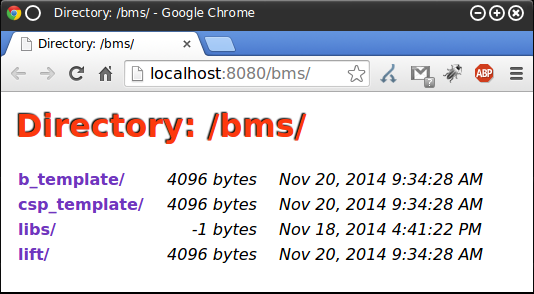
\includegraphics[width=12cm]{img/tutorial/tut_01.png}
	\caption{\bms~Workspace}
	\label{fig_tut_01_workspace}
\end{center}
\end{figure}

\subsection{The Formal Model}

We are going to create a visualisation for a simple lift system that allows movement of a single lift cage between three floors.
The door of the lift can be closed and opened - all in response to the pressing of floor call and cage send buttons.

You can download the Event-B model \file{EventBLift.zip}{here}.
Decompress it and put the files into a new folder called \texttt{model} relative to your \texttt{template.html} file in your workspace.

\subsection{Linking a Model with the Visualisation}

The next step consists of linking the model with the visualisation.
For this, open the \texttt{template.html} file with a text editor of your choice and add the following line within the head tag:

\begin{lstlisting}[language=html]
<meta name="bms.model" content="model/MLift.bcm" />
\end{lstlisting}

We link the visualisation with the Event-B machine called ``MLift''.
Linking a model within the \texttt{template.html} file automatically loads the model, when starting the visualisation.
Your \texttt{template.html} file should look like:

\begin{lstlisting}[language=html]
<html bms-app>
  <head>
      <title>BMotion Studio for ProB</title>
      <meta name="bms.model" content="model/MLift.bcm" />
      <meta name="bms.tool" content="BAnimation" />
      <meta name="bms.script" content="template.groovy" />
      <script src="/bms/libs/requirejs/require.js"></script>
      <script>
        require(['/bms/libs/prob/config.js'], function () {
          require(['template']);
        });
      </script>
  </head>
  <body>
  </body>
</html>
\end{lstlisting}

\info{The meta tag \textit{bms.script} (line 6) contains the link to the Groovy script file and the meta tag \textit{bms.tool} (line 5) defines the formalism or the simulator respectively that should be used. In this case we are creating a visualisation for a ``BAnimation'' (Classical-B or and Event-B).}

\subsection{Creating the Actual Visualisation}

The next step consists of creating the actual visualisation.
The user is not restricted to an editor in order to create a visualisation.
The user can make use of any tool that support the creation of SVG graphics or HTML documents.
For this tutorial we are going to use the Inkspace\footnote{\url{https://inkscape.org}} editor. Inkscape is an editor for creating vector graphics that is available for Windows, Mac OS X and Linux.
It's free and open source.
With Inkscape the user can export the vector graphic into the SVG format.

%\info{We are currently working on a build-in graphical editor for creating SVG graphics and for managing observers.}

\begin{figure}[!ht]
\begin{center}
	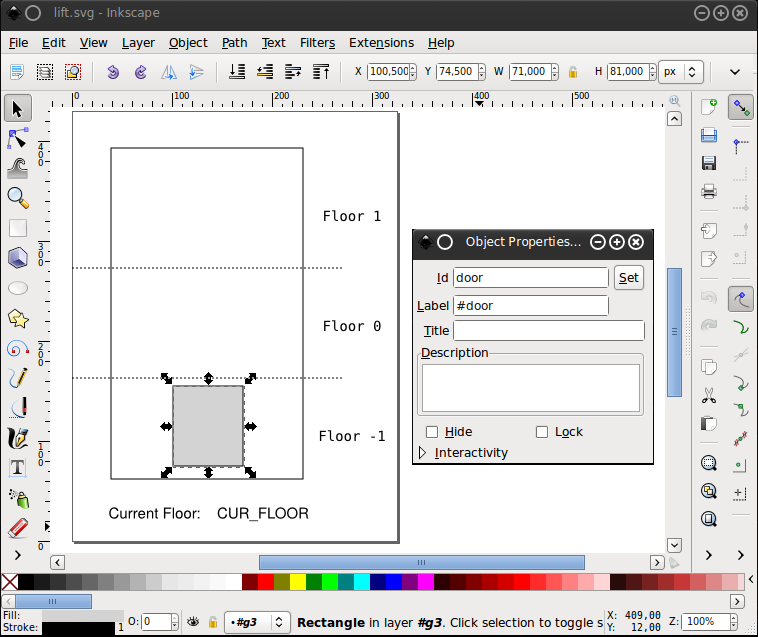
\includegraphics[width=12cm]{img/tutorial/tut_02.png}
	\caption{Creating an SVG graphic with Inkscape}
	\label{fig_tut_02_inkscape}
\end{center}
\end{figure}

%Please download the prepared \file{lift.svg}{lift.svg} file and put it relative to your \texttt{template.html} file in your workspace.
%Add the following tag within the body tag in your \texttt{template.html} file:
%\begin{lstlisting}[language=html]
%<object data="lift.svg" type="image/svg+xml" data-bms="svg">
%</object>
%\end{lstlisting}

Please download the prepared \file{lift.svg}{lift.svg} file and open it with Inkscape as demonstrated in Figure~\ref{fig_tut_02_inkscape}.
Feel free to modify and explore the SVG graphic.
In order to link visual elements of the SVG graphic with the formal model, we have to give them identifiers. 
For this, select an element, open the context menu and select \textsf{Object Properties}.
A popup window should be opened as demonstrated in Figure~\ref{fig_tut_02_inkscape}.
As an example, we give the visual element that represents the door, the id ``door''.
In Section~\ref{sec_creation_observers} we explain how we can use this information in order to create the link between the formal model and the visualisation by means of observers.
If you are satisfied with your SVG graphic, save it as a plain SVG graphic with \textsf{File $\rangle$ Save As}.
Select \textsf{Plan SVG (*.svg)} as an output format and click on the \textsf{Save} button.
You can save the SVG file anywhere on your local system. 
Open the SVG file with a text editor of your choice and put the SVG code within the body tag in the \texttt{template.html} file located in your workspace.
%Your \texttt{template.html} file should look like in Listing~\ref{lst:lifthtml}.

%\begin{lstlisting}[float=ht,language=html, ,caption={Template HTML file with Lift SVG graphic},label=lst:lifthtml]
%<html>
%  <head>
%      <title>BMotion Studio for ProB</title>
%      <meta name="bms.model" content="model/MLift.bcm" />
%      <meta name="bms.tool" content="BAnimation" />
%      <meta name="bms.script" content="template.groovy" />
%      <script data-main="template" src="/bms/libs/requirejs/require.js"></script>
%  </head>
%  <body>
%      <svg width="325" height="430" xmlns="http://www.w3.org/2000/svg">
%            <rect stroke="#000000" id="svg_1" height="331" width="192" y="37" x="39" fill="#ffffff" />
%            <line id="svg_2" y2="267" x2="270" y1="267" x1="0" stroke-dasharray="2,2" stroke="#000000" fill="none" />
%            <line id="svg_4" y2="157" x2="270" y1="157" x1="0" stroke-dasharray="2,2" stroke="#000000" fill="none" />
%            <rect fill="lightgray" stroke="#000000" x="101" y="275" width="70" height="80" id="door" />
%            <text font-weight="normal" xml:space="preserve" text-anchor="middle" font-family="Monospace" font-size="14" id="txt_floor1" y="110" x="280" stroke-dasharray="2,2" stroke-width="0" stroke="#000000" fill="#000000">Floor 1</text>
%            <text id="txt_floor0" font-weight="normal" xml:space="preserve" text-anchor="middle" font-family="Monospace" font-size="14" y="220" x="280" stroke-dasharray="2,2" stroke-width="0" stroke="#000000" fill="#000000">Floor 0</text>
%            <text id="txt_floor-1" font-weight="normal" xml:space="preserve" text-anchor="middle" font-family="Monospace" font-size="14" y="330" x="280" stroke-dasharray="2,2" stroke-width="0" stroke="#000000" fill="#000000">Floor -1</text>
%            <text fill="#000000" stroke="#000" stroke-width="0" x="145" y="407.5" id="txt_cur_floor" font-size="15" font-family="Helvetica, Arial, sans-serif" text-anchor="left" xml:space="preserve">CUR_FLOOR</text>
%            <text fill="#000000" stroke="#000" stroke-width="0" x="36.5" y="407.5" id="svg_3" font-size="15" font-family="Helvetica, Arial, sans-serif" text-anchor="left" xml:space="preserve">Current Floor:</text>
%    </svg>
%  </body>
%</html>
%\end{lstlisting}

\subsection{Starting the Visualisation}

Let's try out the visualisation!
In your browser, navigate to the \texttt{lift} folder and click on the \texttt{template.html} file.

The visualisation should start.
At the right bottom you will find a menu called \textsf{Open View} for opening different ProB related views.
For instance, Figure~\ref{fig_tut_03_running1} shows the running Lift visualisation with the ProB Events view opened.

At the moment nothing spectacular happens when changing the state (i.e. executing events in the Event view), because no link between visual elements and the formal model exists yet.
In the next Section we learn creating observers.

\begin{figure}[!ht]
\begin{center}
	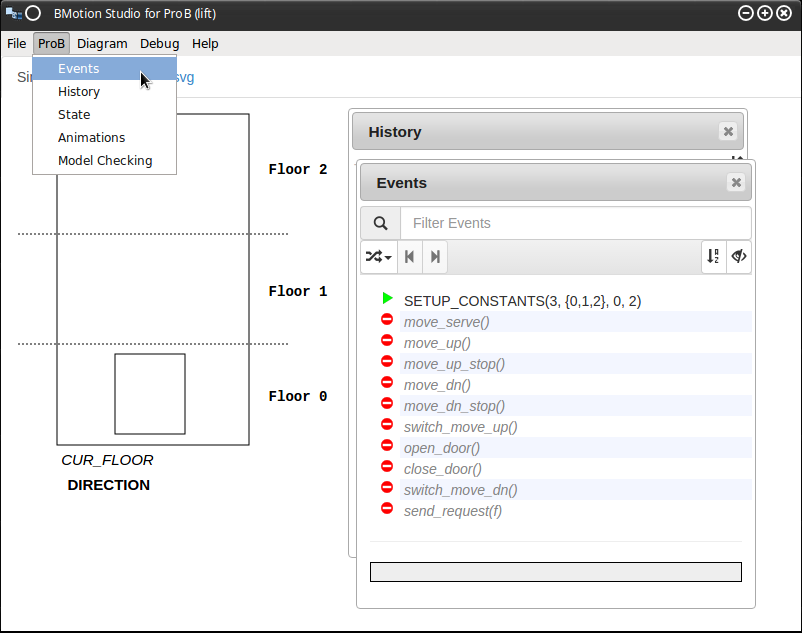
\includegraphics[width=12cm]{img/tutorial/tut_03.png}
	\caption{Running the Lift Visualisation for the First Time}
	\label{fig_tut_03_running1}
\end{center}
\end{figure}

\subsection{Creating Observers}
\label{sec_creation_observers}

Observers are used to link visual elements with the model. 
An observer is notified whenever a model has changed its state, i.e. whenever an event has been executed. 
In response, the observer will query the model's state and triggers actions on the linked visual elements in respect to the new state.
As an example, consider the following observer written in JavaScript:

\begin{lstlisting}[float=ht,language=JavaScript, caption={Formula Observer Displaying the Current Floor (JavaScript)}]
$("#txt_cur_floor").observe("formula", {
  formulas: ["cur_floor"],
  trigger: function (origin, data) {
    origin.text(data.values[0].value)
  }
});
\end{lstlisting}

We are going to explore the JavaScript code line by line.
In line 1 we register a formula observer on the visual element with the id \textit{txt\_cur\_floor} that is located in our \texttt{template.html} file.
%Line 1 means that we want to transform the visual element with the id \textit{txt\_cur\_floor} that is located in our \texttt{template.html} file.
\bms~follows the jQuery selector syntax\footnote{\url{http://api.jquery.com/category/selectors}} to select elements.
The prefix ``\#'' denotes that we want to select an element by its id.
In line 2 we define a list of observed formulas.
In this case we observe the variable \textit{cur\_floor}.
In line 3 to 5 we define a trigger function that is called after every state change with its \textit{origin} reference to the element that the observer is attached to and the requested \textit{data} (the result of the formulas).
The function changes the text of the element to the current value of the variable \textit{cur\_floor}.
%Line 2 affects that the attribute \textit{text} will be set to the value that is returned by the followed closure.
%In particular, the closure evaluates the expression \textit{cur\_floor} in the current state and returns the value to be set.
%In other words, the observer sets the current value of the variable \textit{cur\_floor} into the visual text element with the id \textit{txt\_cur\_floor}.
%Line 3 is responsible to register the observer.
%All registered observer will be triggered after every state change.

Let's create another observer.
Check out the following code:

\begin{lstlisting}[float=ht,language=JavaScript, caption={Formula Observer for the Lift Door (JavaScript)}]
$("#door").observe("formula", {
  formulas: ["cur_floor", "door_open"],
  trigger: function (origin, data) {
    
    switch (data.values[0].value) {
      case "0":
        origin.attr("y", "175");
        break;
      case "1":
        origin.attr("y", "60");
        break;
      case "-1":
        origin.attr("y", "275");
        break;
    }
    
    if(data.values[1].value === "TRUE") {
      origin.attr("fill", "white");
    } else {
      origin.attr("fill", "lightgray");
    }
    
  }
});
\end{lstlisting}

In line 1 we register a formula observer on the visual element with the id \textit{door}, similar to the previous defined observer.
%Line 1 means that we want to transform the visual element with the id \textit{door}, similar to the previous observer.
In line 2 we define the set of observed formulas (\textit{cur\_floor} and \textit{door\_open}).
In line 3 to 23 we define a trigger function.
In particular, line 5 to 15 will switch the \textit{y} coordinate of the door (denoting the movement of the door between floors) according to the current value of the variable \textit{cur\_floor}.
Lines 17 to 21 affect that the attribute \textit{fill} of the door will be set to ``white'' (denoting the door is open) whenever the formula \textit{door\_open} evaluates to \textit{TRUE} in the current state, otherwise to ``lightgray'' (denoting the door is closed).
%Whenever the expression \textit{door\_open} evaluates to \textit{TRUE}, the value \textit{white} (denoting the door is opened) is returned, otherwise the value \textit{lightgray} (denoting the door is closed) is returned.
%Line 3 to 17 will switch the \textit{y} coordinate of the door (denoting the movement of the door between floors) according to the evaluation result of the expression \textit{cur\_floor}.
%In line 18 we register the observer.
%You can use the entire Groovy power and feature range for defining your observers.

Add both snippets to your \texttt{template.js} file and refresh your browser.
Let's see how this affects the visualisation:
Setup and initialise the machine using the ProB events view.
Execute some events and see what happens.
For instance, Figure~\ref{fig_tut_04_running2} shows the lift visualisation where the lift is on floor 0 and the door is open.

\begin{figure}[!ht]
\begin{center}
	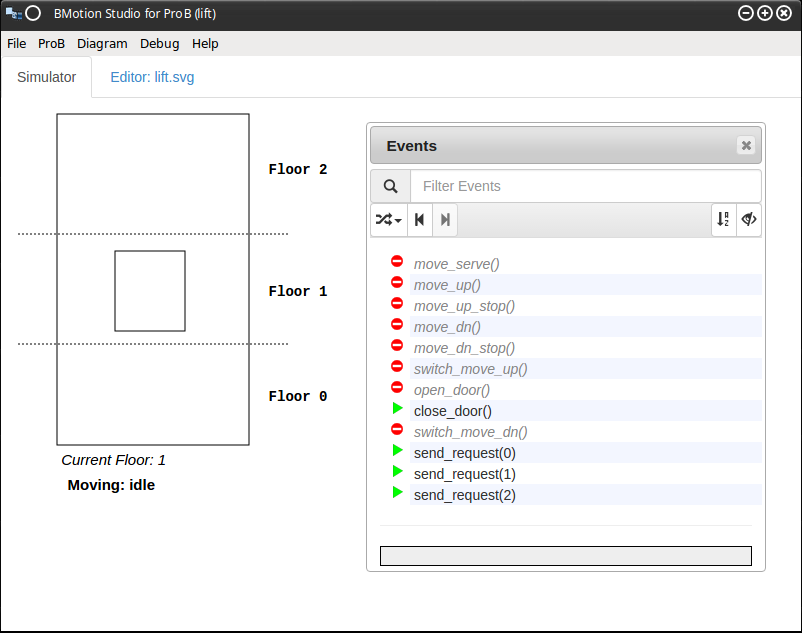
\includegraphics[width=12cm]{img/tutorial/tut_04.png}
	\caption{Lift Visualisation with Transformer Observer}
	\label{fig_tut_04_running2}
\end{center}
\end{figure}

\subsection{Add Interactivity}

In this Section we learn how we can enhance our visualisation with interactive features, like executing some Event-B events by clicking on some buttons.

Let's add an interactive feature, where the user can click on a floor label to order the lift on the corresponding floor.
Add the code snippet to your \texttt{template.js} file:
\newpage
\begin{lstlisting}[language=JavaScript, caption={Example of an Interactive Feature (JavaScript)}]
$("text[data-floor]").executeEvent({
  events: [
    {
      name: "push_call_button", 
      predicate: function (origin) {
        return "b=" + $(origin).attr("data-floor")
      }
    }
  ]
});
\end{lstlisting}
%For instance, clicking on the floor Label ``Floor 1'' should execute the Event-B event \textit{push\_call\_button(1)}.
In line 1 we register an execute event handler for each visual element that matches the defined selector ``text[data-floor]''.
In particular, the selector matches the three floor labels (see Figure~\ref{fig_tut_03_running1}).
In line 2 to 15 we define the event that should be executed after clicking on the corresponding floor label.
We use the content of the attribute \textit{data-floor} of the corresponding floor label (\textit{origin}) in order to define the parameter/predicate.

Apply these changes by refreshing your browser and try to click on a floor label.
This should call the Event-B event \textit{push\_call\_button} with the corresponding predicate/parameter.

Let's add another interactive feature, where the user can click on the visual element that represents the door to open or close the door respectively.
%The first step consists of registering a new Groovy function that executes the corresponding event \textit{open\_door} or \textit{close\_door}.
%Add the code snippet to your \texttt{template.groovy} file:
%\begin{lstlisting}[language=Groovy, caption={Registering a Groovy Function (Groovy)}]
%bms.registerMethod("openCloseDoor", {
%    def Trace t = bms.getTool().getTrace()
%    def Trace newTrace = executeEvent(t, "open_door", []) ?: executeEvent(t, "close_door", [])
%    if (newTrace != null) {
%        animations.traceChange(newTrace)
%        return [newState: newTrace.getCurrentState().id]
%    }
%})
%
%def Trace executeEvent(t,name,pred) {
%    try {
%        t.execute(name, pred)
%    } catch(IllegalArgumentException e) {
%        null
%    }
%}
%\end{lstlisting}
%In Line 1 we register a new Groovy function called \textit{openCloseDoor}.
%The next lines show an example how we can use the ProB Java API.
%In Line 2 we get the current trace of the animation.
%In Line 3, we first try to execute the \textit{open\_door} event by means of a helper method called \textit{executeEvent} (Line 10 to 16).
%If the return value of the helper method is null (the event could not be executed), we try to execute the event \textit{close\_door}.
%If we success (we executed one of the both events), we trigger a trace change, causing to refresh the current animation (Line 5).
%This in turn changes the state and triggers our registered observers.
%Line 6 returns a Json object that contains the state id of the new state.
%This information can used later at the JavaScript side after executing the registered \textit{openCloseDoor} method.
%Let's switch to the JavaScript side.
Add the following code snippet to your \texttt{template.js} file:
%\begin{lstlisting}[language=JavaScript, caption={Call openCloseDoor Groovy Method (JavaScript)}]
%$("#door").click(function () {
%	bms.callMethod("openCloseDoor", {
%		callback: function (data) {
%			console.log("Callback: " + data)
%		}
%	})
%}).css("cursor", "pointer")
%\end{lstlisting}
\begin{lstlisting}[language=JavaScript, caption={Interaction with the Lift Door (JavaScript)}]
$("#door").executeEvent({
  events: [
    { name: "close_door" }, 
    { name: "open_door" }
  ],
  callback: function (data) {
    console.log("Callback: " + data)
  }
});
\end{lstlisting}

In line 1 we register a new execute event handler on the visual element with the id door.
The execute event handler first tries to execute the event \textit{open\_door}.
In case the event is disabled, it tries to execute the next event \textit{close\_door}.
%Line 2 calls our registered Groovy method \textit{openCloseDoor}.
In Line 3 to 5 we pass a callback function that is called after an event (\textit{open\_door} or \textit{close\_door}) was executed.
%In this case we print the returned new state id on the console.

These are only small examples for adding interactivity to your visualisation.
You are not limited to these examples.
You can download the final visualisation \file{LiftVisualisation.zip}{here}.




\chapter{Reference}
\label{reference}

\section{The BMotion Studio API}
\label{sec:bmsapi}

(tbd)

\section{Observers}
\label{sec:observers}

Observers are used to link visual elements with the model. 
An observer is notified whenever a model has changed its state, i.e. whenever an event has been executed. 
In response, the observer will query the model's state and triggers actions on the linked visual elements in respect to the new state. 

\subsection{Observers in Groovy}
\label{sec:groovy_observers}

In general, observers are defined in the Groovy script file.
\bms~comes with some predefined observers that are described in the following sections.

\subsubsection{Transformer Observer}
\label{sec:transformer_observer}

The transformer observer supports changing attributes of visual elements based on the current state of the animation.
The following code snippet demonstrates the basic use of a transformer observer:

\begin{lstlisting}[float=ht,language=Groovy]
transform("#myvisualelement") {
    set "fill", "green"
    set "stroke", "red"
    register(bms)
}
\end{lstlisting}

In line 1 we define a jQuery selector to select the visual elements which should be transformed.
In this case we select a visual element with the id \textit{myvisualelement} (in jQuery the prefix ``\#'' denotes that we want to select and element by its id).
jQuery provides several possibilities to select visual elements.

\info{The jQuery selector API documentation\footnote{\url{http://api.jquery.com/category/selectors/}} provides an overview and a detailed documentation about selectors.}

Line 2 to 3 are actions that are made on the visual elements which are matched by the defined selector.
In this case the \textit{fill} attribute is set to the value \textit{green} and the \textit{stroke} attribute to \textit{red}.

In line 4 we register the observer to the current visualisation.
A registered observer is triggered after every state change, e.g. after executing an event.

\paragraph{Groovy Closures.}
%As we use the Groovy Scripting language for defining the observers, we can make use of the entire function and feature range of it.
Transformer observers supports the use of Groovy closures for defining the selector or the value of an action.

The following code snippet demonstrates the use of closures for transformer observers:

\begin{lstlisting}[float=ht,language=Groovy]
transform("#myvisualelement") {
  set "fill", { (bms.eval("1 < x").value == "TRUE") ? "white" : "lightgray" }
  set "y", {
    switch (bms.eval("x").value) {
      case "0": "15"
        break
      case "1": "20"
        break
      case "2": "25"
        break
      default: "0"
    }
  }
  register(bms)
}
\end{lstlisting}

In Groovy a closure is encapsulated in curly brackets.
Line 2 and 3 show two examples for using closures for defining the value of the attribute \textit{fill} and \textit{y} respectively.
Closures are evaluated after every state change in consequence of triggering the transformer observer.
As an example, in line 2 the closure evaluates the expression $1 < x$.
The value of the \textit{fill} attribute is set to \textit{white} whenever the expression evaluates to \textit{TRUE} and otherwise to \textit{lightgray}.


\subsubsection{Method Observer}
\label{sec:method_observer}

The following code snippet gives an example of the method observer:

\begin{lstlisting}[float=ht,language=Groovy]
callMethod("mymethod") {
  data([foo: "bar"])
  register(bms)
}
\end{lstlisting}

\subsubsection{Custom Observer}
\label{sec:custom_observers}

The following code snippet gives an example of a custom observer:
\begin{lstlisting}[float=ht,language=Groovy]
def customObserver = [ 
  apply: { bms ->  println "Triggering custom observer." } 
] as BMotionObserver
bms.registerObserver(customObserver)
\end{lstlisting}

You can also create a custom transformer observer:
\begin{lstlisting}[float=ht,language=Groovy]
def transformerObserver = [
  update: { bms ->
    def transformers = []
    def result = bms.translate("relation")					
    result.value.each { obj ->
      transformers += transform("#" + obj.first) {
        set "transform", "translate(" + obj.second + ")"
        update(bms)
      }
    }
    return transformers
  }
] as BMotionTransformer
bms.registerObserver(transformerObserver)
\end{lstlisting}

\subsection{Observers in JavaScript}
\label{sec:js_observers}

The user can add an observer in JavaScript by means of the \textit{bms} API variable. An example:

\begin{lstlisting}[float=ht,language=JavaScript]
bms.observe({
  expressions: ["floor", "x>4"],
  trigger: function (data) {
  	var el = $("#myvisualelement")
    el.html(data.values[0].value)
    if(data.values[0].value === "TRUE") {
      el.attr("fill","green")
    } else {
      el.attr("fill","red")
    }
  }
});
\end{lstlisting}

The user can also assign an observer to an selector object:

\begin{lstlisting}[float=ht,language=JavaScript]
$("#door").observe({
  expressions: ["cur_floor", "door_open"],
  trigger: function (origin, data) {
    var values = data.values
    switch (values[0].value) {
      case "-1": origin.attr("y", "275"); break
      case "0": origin.attr("y", "175"); break
      case "1": origin.attr("y", "60"); break
    }
    values[1].value === "TRUE" ? origin.attr("fill", "white") : origin.attr("fill", "lightgray")
})
\end{lstlisting}


\chapter{Frequently Asked Questions}
\label{faq}

\section{General Questions}

\subsection{What is BMotion Studio?}

Text ...


\clearpage
\phantomsection
\addcontentsline{toc}{chapter}{Index} 
\printindex

\end{document}

